\newpage
\subsection{Поступление материалов}
\label{bp:MatInput}
%


\subsubsection{Поступление бумаги и картона}

Рулоны бумаги и картона принимаются кладовщиками на склад ролевой продукции. Поступление рулонов по датам контролируется кладовщиками на основании документа ''Заказ поставщику'' (рис. \ref{pic:IX.1..}) в системе 1С: УПП. Макулатурное сырье поступает с ООО ''ПЗБМ''. Целлюлозное сырье поступает от сторонних производителей АО ''АЦБК'' и  АO ''CЛПК''.
Проезд автотранспорта на территорию ПРЕДПРИЯТИЯ для погрузки или разгрузки осуществляется после оформления в системе 1С: УПП документа ''Проездной лист'' (рис. \ref{pic:IX.2}).
Кладовщик принимает машину с рулонами. Кладовщик принимает рулоны бумаги и картона по отвес-фактуре поставщика по номерам рулонов.  

В системе 1С: УПП при приемке сырья ООО ''ПЗБМ'' создается документ ''Приходный ордер на товары'' (приход по сериям) и серии номенклатуры не присваиваются (рис. \ref{pic:IX.1....}), т.к. они уже указаны. При поступлении целлюлозного сырья в системе 1С: УПП также создается ''Приходный ордер на товары'' (приход прочие), но создаются серии номенклатуры и проставляются форматы (рис. \ref{pic:IX.1,}).
На основании документов ''Приходный ордер на товары''  в системе 1С: УПП кладовщик создает документы ''Поступление товаров и услуг'' и распечатывает их. 
%Рулон принимается на склад в любом случае.

%Кладовщик заносит поступление рулонов в системе СБИС в документ ''Приходная накладная'' .
%Если качество рулона при приемке совсем не соответствует заявленному, то кладовщик составляет акт Торг-2 на возврат, но все равно принимает на склад.

%Учет бумаги и картона выполняется в метрах квадратных и в количестве рулонов в системе СБИС по номера рулонов.

Кладовщики при приемке рулонов бумаги и картона указывают поступление в тоннах.
Кладовщик передает документы по поступлению сырья в бухгалтерию ежедневно.

 %Бухгалтер на основе приходных документов от поставщика в системе СБИС находит документ поступления, заполняет цены на сырье из сопроводительных документов и проводит документ.
Рулоны от  АО ''АЦБК'' и  АO ''CЛПК'' принимаются совместно с ОУК. Если рулон имеет дефекты (поврежден), то он принимается в любом случае. ОУК оформляет акт. Рулон вскрывается в присутствии учетчика, старший машинист гофроагрегата (обер) определяет сколько требуется срезать брака с рулона. После того как брак срезан, рулон после взвешивания принимается на склад с новым весом. 

Для контроля остатков кладовщики используют различные отчеты в системе 1С: УПП. 
Адресного хранения рулонов на складе нет, но водители погрузчиков стараются ставить рулоны по форматам (рис. \ref{pic:IX склад сырья}). Где находятся конкретные рулоны, знают только водители погрузчиков.
% \subsubsection{Поступление рулонов бумаги и картона}

% Не производится.

% В форме к системе 1С 8 ''Управление торговлей'' ведутся данные по движению рулонов между площадками производство. В системе 1С 8 ''Управление торговлей'' данные по движению рулонов оперативны и достоверны.

% Диспетчер сообщает кладовщику о поступлении машины кладовщику. Кладовщик принимает машину с рулонами. Кладовщик принимает рулоны бумаги и картона по отвес-фактуре по номерам рулонов.  Кладовщик производит первичный осмотр качество рулонов, производит отбраковку в случае необходимости. Дефект рулона чаще всего связан с неправильной транспортировкой.  При необходимости кладовщик составляет акт дефектовки рулона. На каждую машину кладовщик составляет заключение по входному контролю качества сырья по  форме \ref{pic:pic_d49.1}.  На основании входного контроля старший кладовщик ведет журнал учета поврежденных рулонов (рис. \ref{pic:pic_d49.1}), которые будут списаны в производство в любом случае.  Входной контроль качества кладовщик передает в отдел технического контроля. Кладовщик передаёт накладную старшему кладовщику.   Комплект документов старший кладовщик передает в бухгалтерию, где заносят поступление сырья в систему 1С 8.3 ''Управление торговлей''. Остатки по сырью бумага и картон достоверные в системе 1С 8.3 ''Управление торговлей''. При этом кладовщик всё равно создает вручную отчет по остаткам (рис. \ref{pic:pic_d25}). Кладовщик каждый день пересчитывает остатки по рулонам. Расхождение могут быть один раз в месяц.


\subsubsection{Поступление прочих материалов}

При поступлении на склад материалов (крахмал, каустик и пр.) оформляется в системе 1С: УПП  документами ''Приходный ордер на товары'', которые создаются на основании документа ''Заказ поставщику''. 








\clearpage
\clearpage
\begin{figure}
\begin{center}
 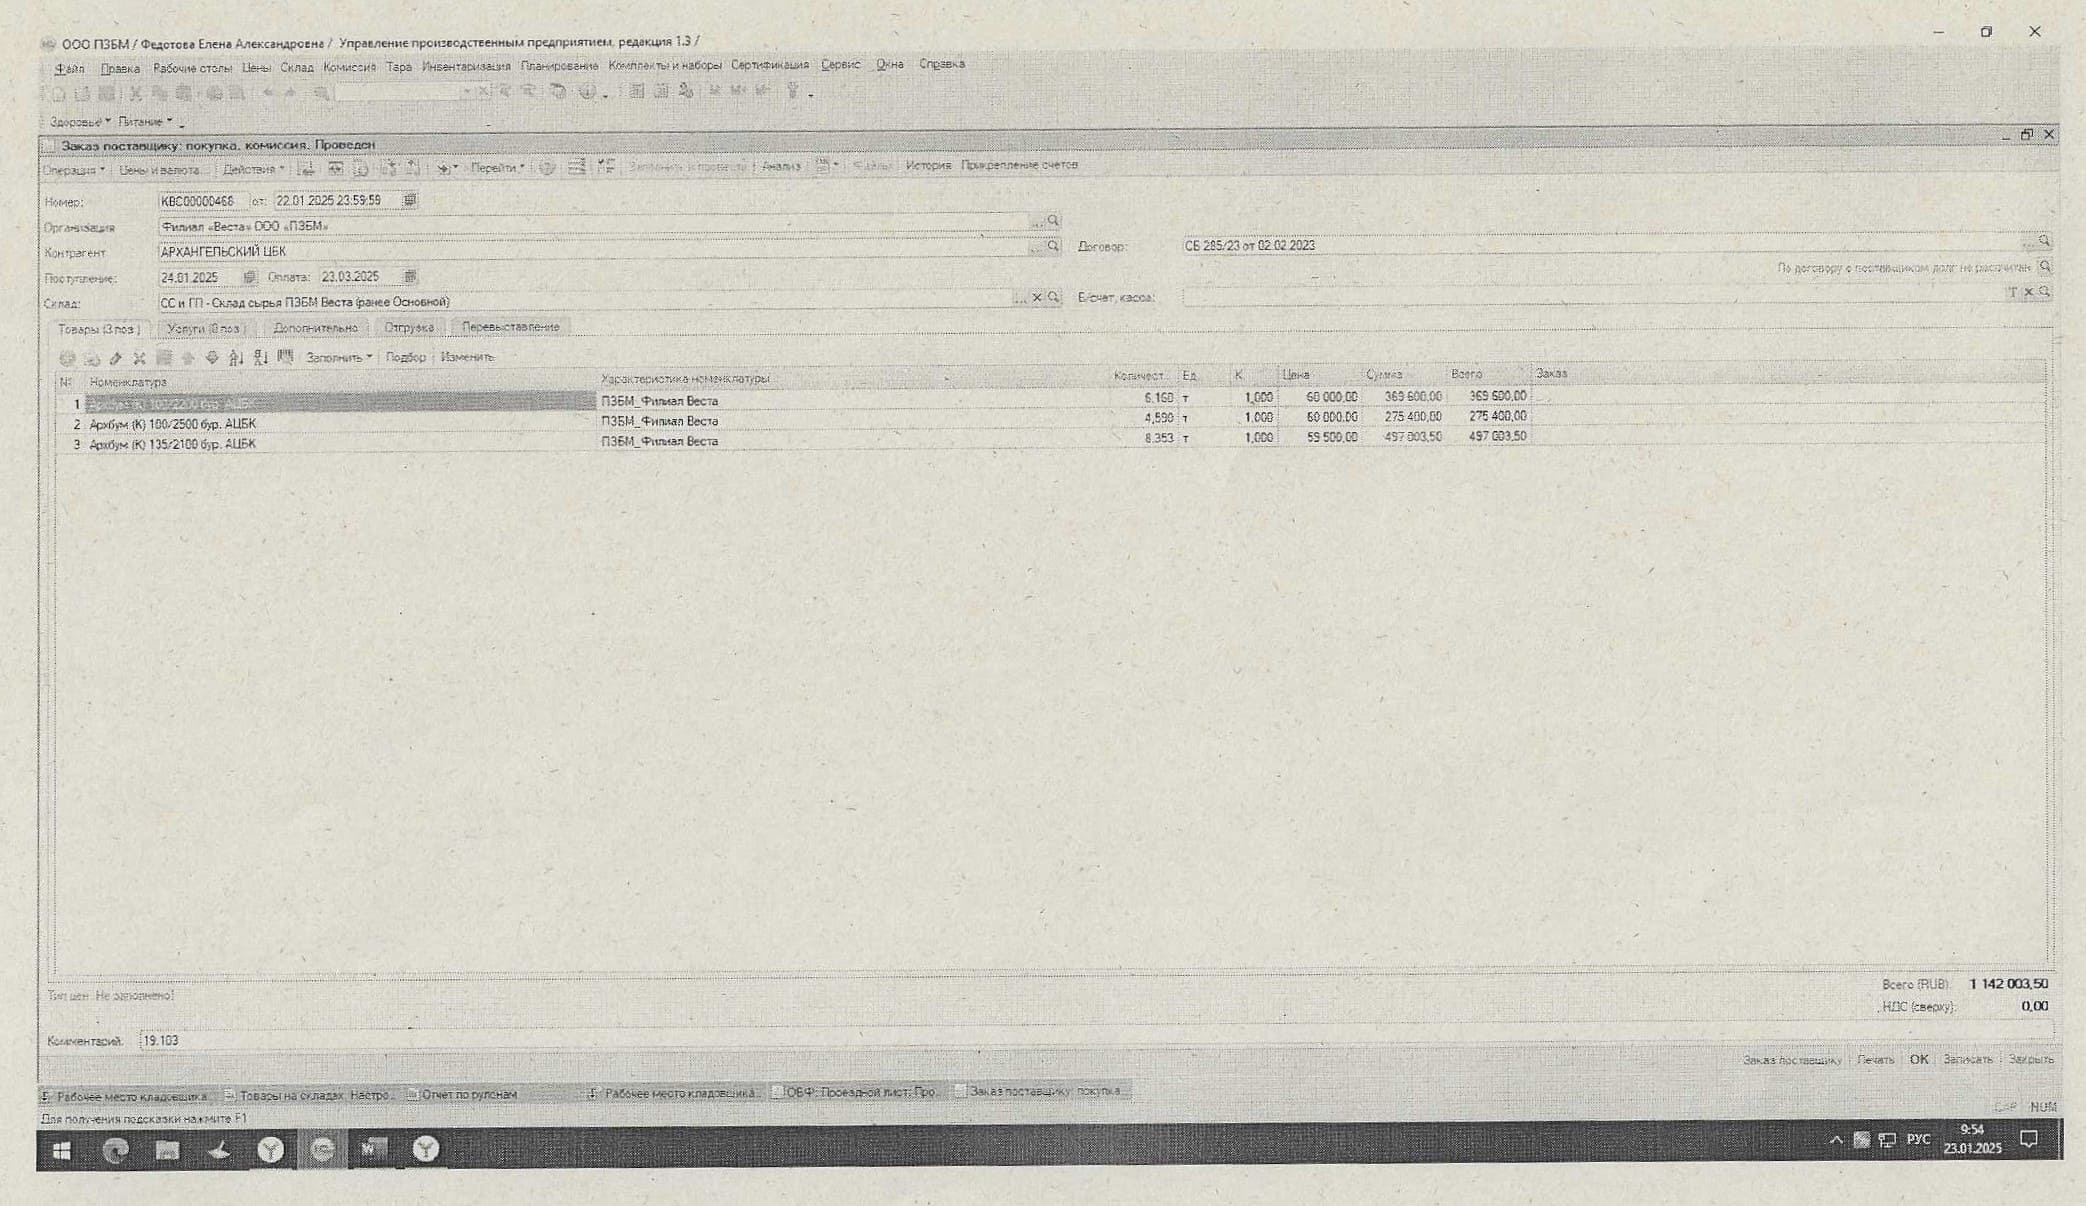
\includegraphics[height=0.39\textheight, keepaspectratio]{Pics/IX.1...jpg}
\end{center}
 \caption{Заказ поставщику}
 \label{pic:IX.1..}
\end{figure}

\begin{figure}
\begin{center}
 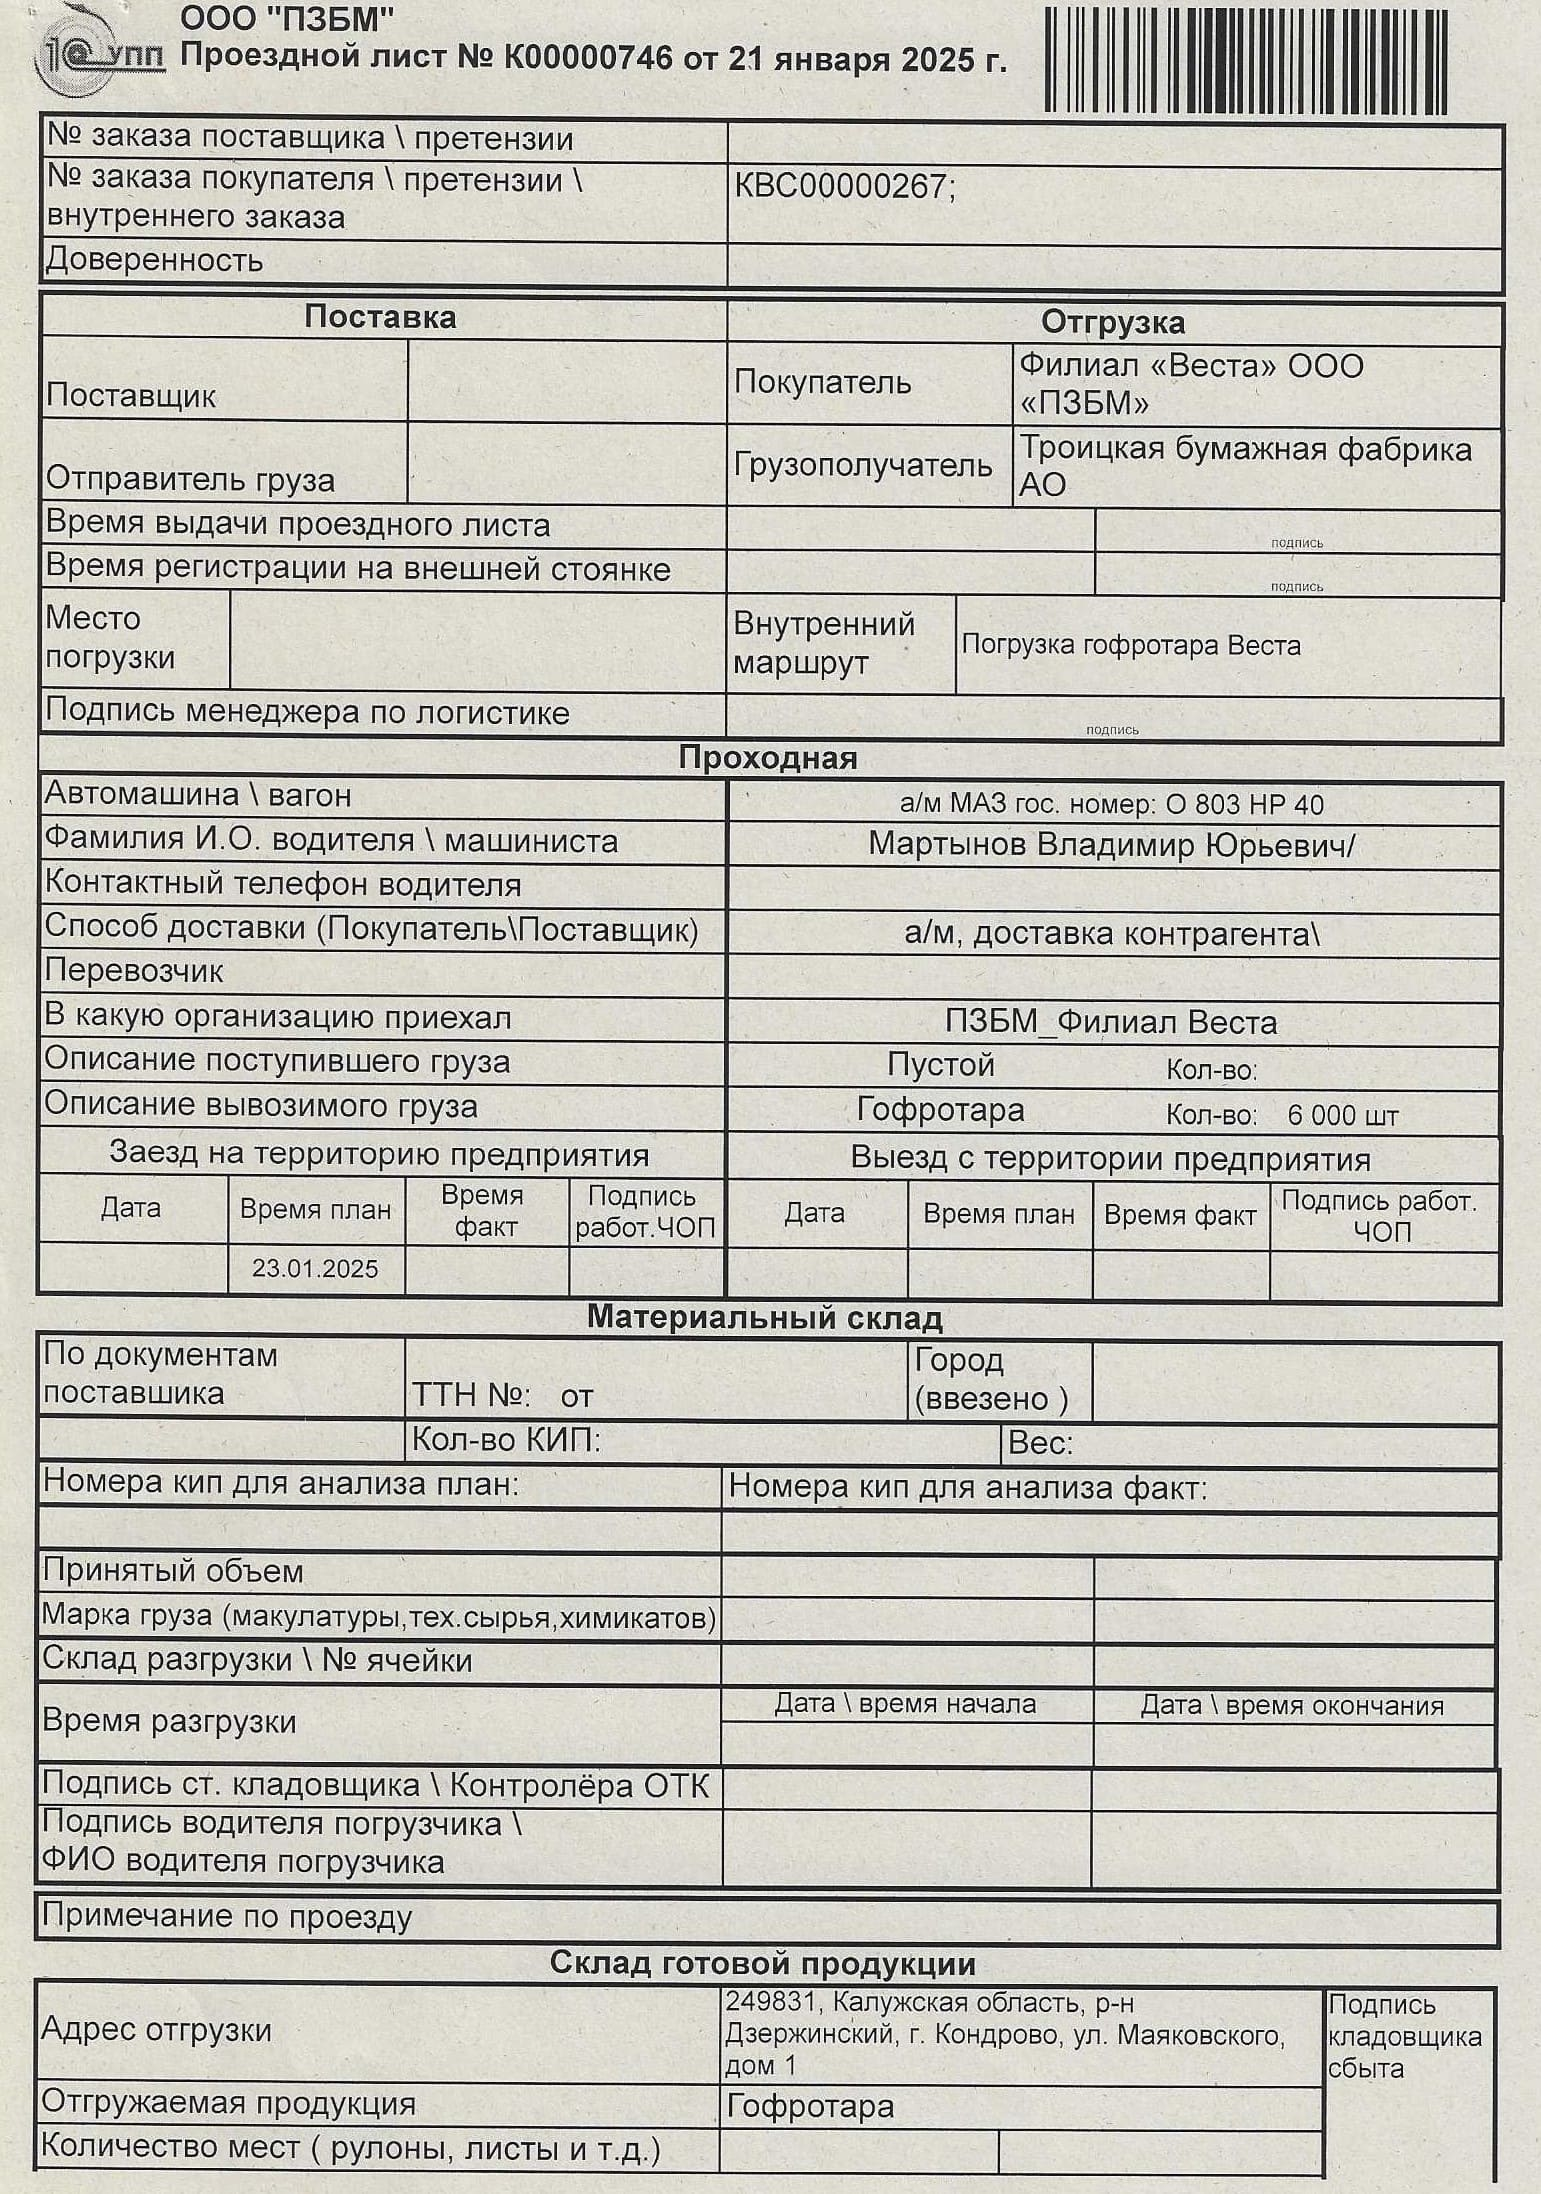
\includegraphics[height=0.9\textheight, keepaspectratio]{Pics/IX.2.jpg}
\end{center}
 \caption{Проездной лист}
 \label{pic:IX.2}
\end{figure}

\begin{figure}
\begin{center}
 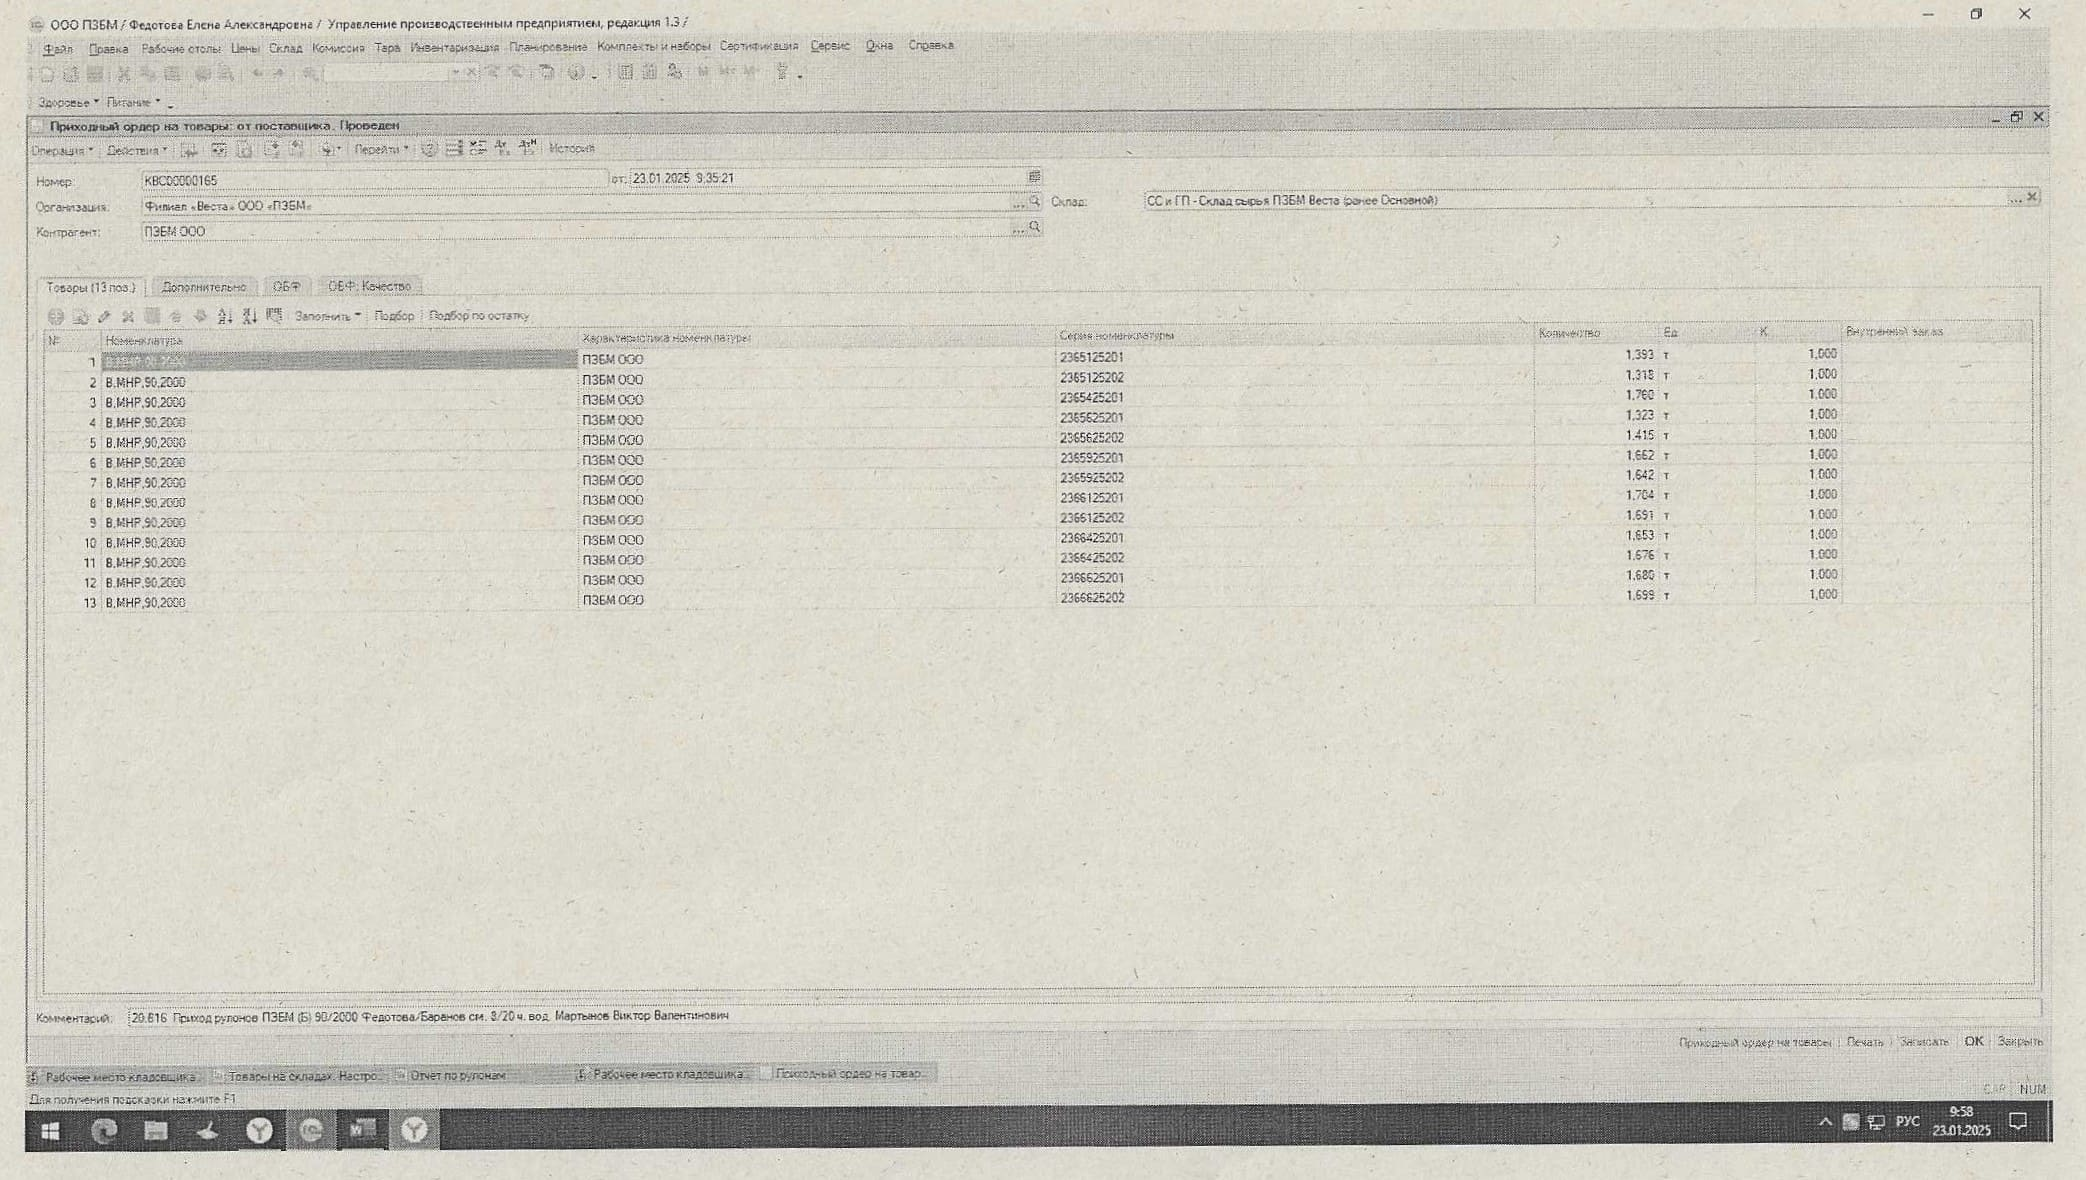
\includegraphics[height=0.38\textheight, keepaspectratio]{Pics/IX.1.....jpg}
\end{center}
 \caption{Приемка рулонов ПЗБМ}
 \label{pic:IX.1....}
\end{figure}

\begin{figure}
\begin{center}
 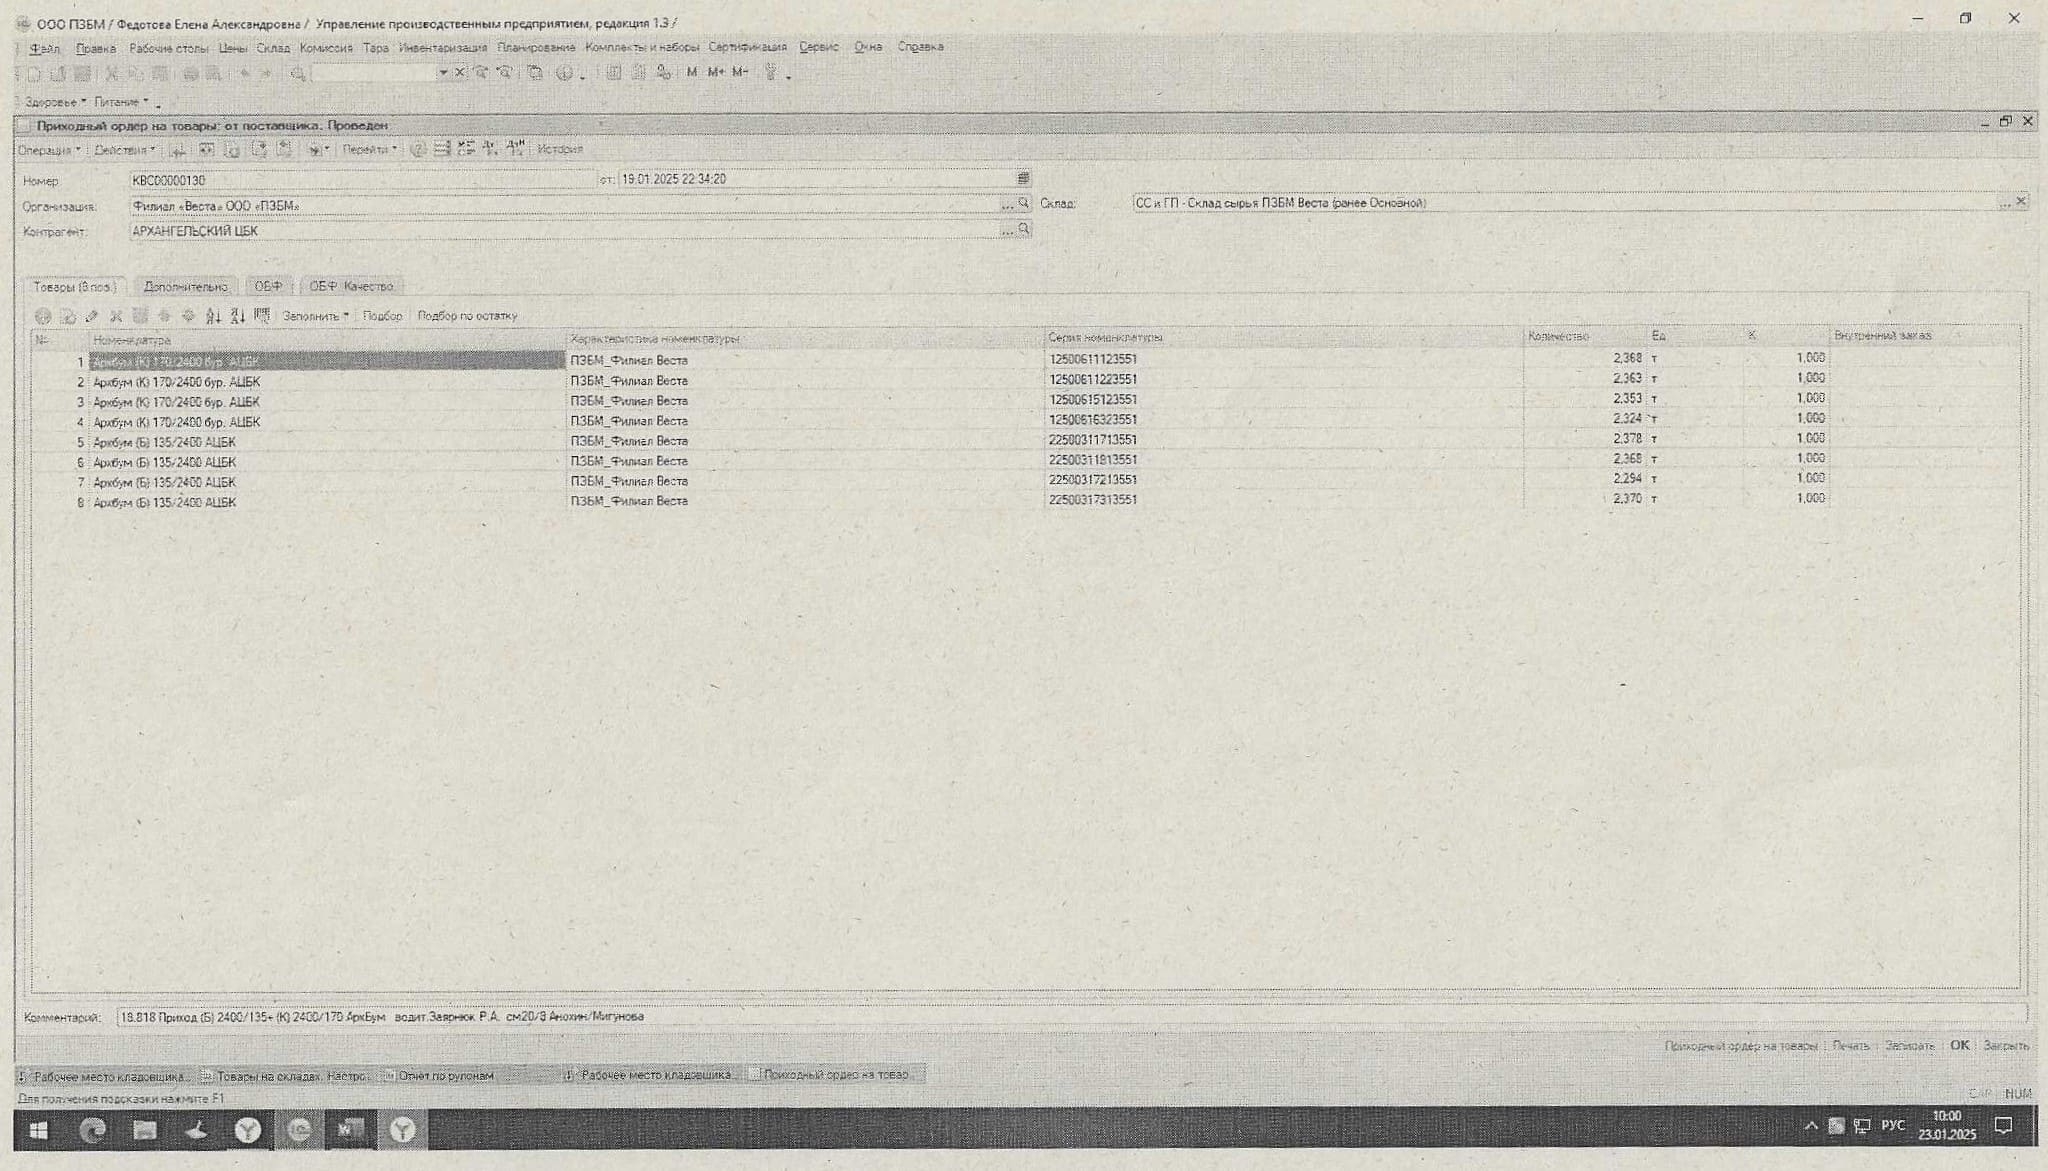
\includegraphics[height=0.38\textheight, keepaspectratio]{Pics/IX.1,.jpg}
\end{center}
 \caption{Приемка рулонов АЦБК}
 \label{pic:IX.1,}
\end{figure}

\begin{figure}
\begin{center}
 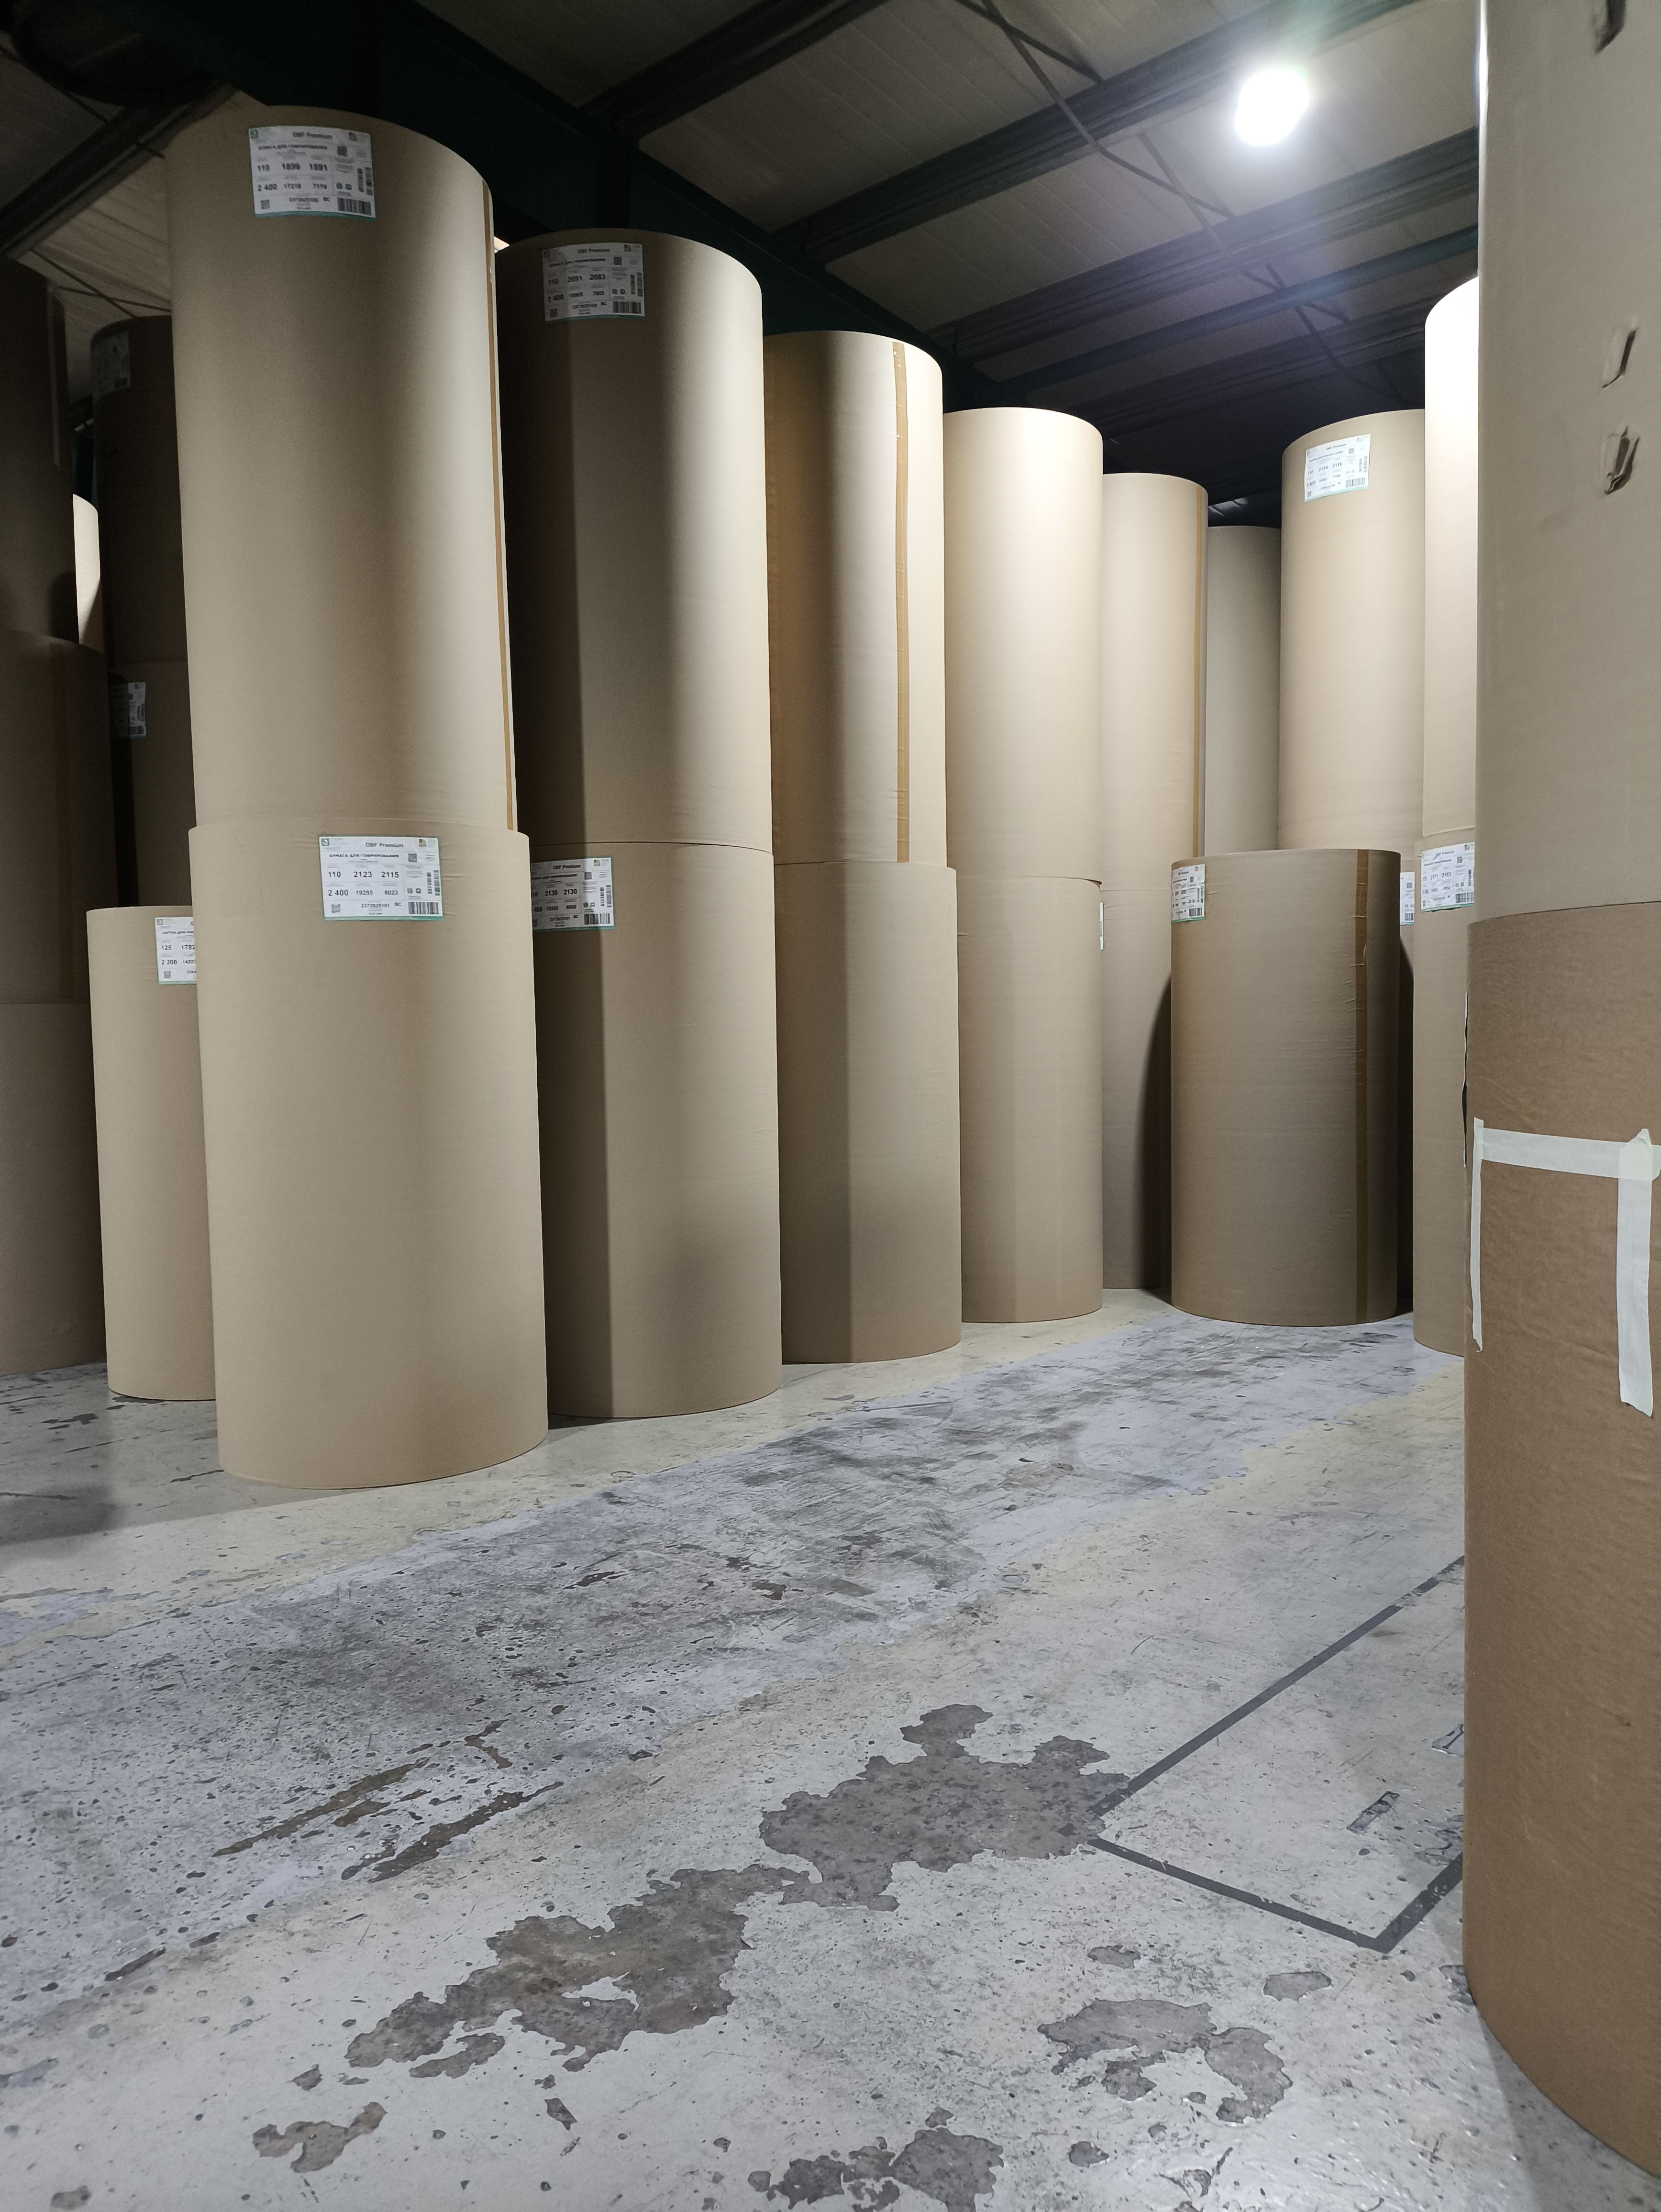
\includegraphics[height=0.9\textheight, keepaspectratio]{Pics/IX склад сырья.jpg}
\end{center}
 \caption{Склад рулонов}
 \label{pic:IX склад сырья}
\end{figure}
% Поступившую краску принимает мастер и  ставит в специально отведенное место для хранения (рис. \ref{pic:a12}). 

% Вспомогательные материалы (клей, лента и пр) кладовщик принимает на склад согласно документам поступления. 
% Полученные накладные кладовщик передает в бухгалтерию, где бухгалтер оприходует материалы в системе 1С:УНФ документом «Поступление ТМЦ». 

% \begin{figure}
% \begin{center}
%   
\includegraphics[height=0.94\textheight, width=\textwidth, keepaspectratio]{Pics/Pattern.jpg}
% \end{center}
%   \caption{Акт о выявлении несоответствия}
%   \label{pic:a61}
% \end{figure}




\clearpage
\ifx \notincludehead\undefined
\normalsize
\end{document}
\fi